%# -*- coding: utf-8-unix -*-

\chapter{机票推荐中的冷启动问题}
\label{chap:cold}

冷启动问题一般分为物品冷启动和用户冷启动。前者的含义是当一件物品新添加到物品库中,在还没有用户使用过的情况下如何将其推荐给用户;后者的含义是当一名新用户来到推荐系统,在完全没有用户偏好的情况下如何为用户推荐适当的物品。冷启动问题是推荐系统需要面对的严峻问题。如果处理不好冷启动问题,系统内添加的新物品可能永远都无法向用户推荐;也会影响到新用户的体验,造成用户流失。\par
在机票推荐系统中,由于机票的数量非常有限并且每条航线上的航班较为固定,通常不会面临物品冷启动问题。而机票本身属于低频、刚需物品。因此机票推荐系统面临的主要问题是用户冷启动问题。在传统的推荐系统中,有一些办法可以解决用户冷启动问题:如在电子商务、书籍网站,用户往往会先提供物品的类别、品牌等信息,随后可以将类别下购买人数的商品推荐给新用户;而在视频、新闻等内容网站,可以在新用户注册时让用户勾选一些感兴趣的主题,即使没有有效获取用户的偏好主题,仍可以将总体最热门的、最实时的内容呈现给用户。\par
在机票推荐研究领域,由于其业务的特殊性,这两种做法均有不足之处。由于机票具有动态属性,难以静态地描述;并且每个航班的机票数量最多在一两百左右,造成的结果是热门物品与冷门物品之间的差别很小。因此很难单纯以热门程度进行推荐。在第三章,图\ref{fig:res_pref_rec}中的结果表明,以航班热门程度排序的策略难以表现出好的推荐效果。其次,影响用户购买决策的因素有很多,用户每次选购机票时注重的属性可能会因为用户的日程安排、出行目的的不同而发生变动。而在内容网站,用户的兴趣主题一般不会发生频繁变动。因此我们需要对冷启动问题展开深入研究。


\section{冷启动用户数据分析}
本小节我们主要对机票推荐中冷启动问题对推荐结果带来的负面影响进行分析与阐述。此处我们仍然选取第三章中提到的四条热门航线进行分析。我们在第三章中提出的机票推荐算法首先将用户数据按照航线进行分割。并为每个用户在每条他选购过机票的航线上独立维护一个偏好表示模型。这样的做法细化了推荐粒度,使用与目标推荐航线相同的航线来进行建模可以得到更贴合的用户偏好。但是用户的历史订单数据却分散到各个航线。如果在待推荐航线上的训练数据过少,则难以精确刻画用户的偏好。在此,我们首先分析航线间的差异,与相似度衡量方法;并分析按航线为用户提取偏好对推荐效果带来的影响。

一堆展开,按捺不住洪荒之力了。

\begin{itemize}
	\item 航线间分布差异、信息熵;航线间相似度衡量;
	\item 分航线偏好和聚合偏好对推荐效果的影响;
	(直方图:当用户在本航线上有几单时,分航线更好,引出活跃用户的概念)
\end{itemize}




图\ref{fig:user_user_percent}的统计结果表明,在北京-上海这条热门程度很高并且订单、用户数量比最高的航线上,平均每位用户的订单数量仅为两单,仍有$60\%$的用户在过去两年仅订过一单,$90\%$的用户仅订过不多于四单。订单数量在四单及以下的用户占了订单总数的$60\%$。

\begin{figure}
 \centering
 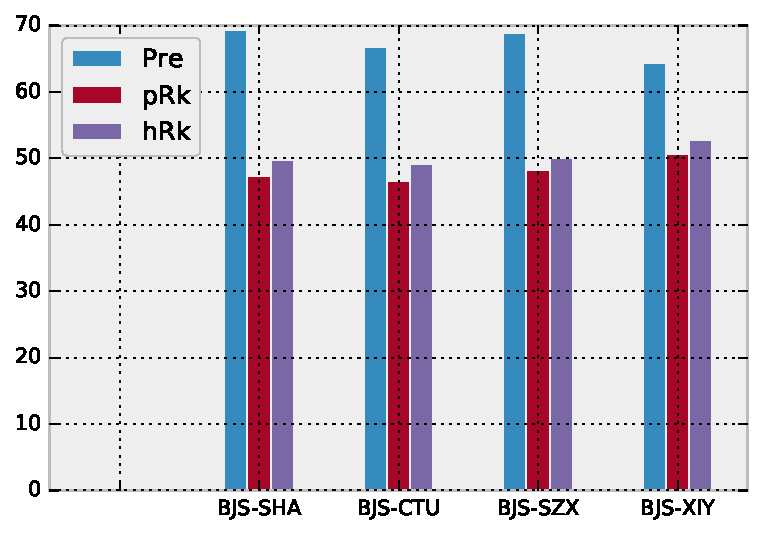
\includegraphics[width=0.9\linewidth]{03/5_res_of_rec.pdf}
 \bicaption[fig:active_inactive_rec]{两类用户推荐效果对比}{活跃用户与非活跃用户的推荐效果对比}{Fig}{Mean Accuracy of Recommendation for Active Users and Inactive Users}
\end{figure}\par

图\ref{fig:active_inactive_rec}展示了在四条热门航线上分别针对活跃用户和
非活跃用户进行机票推荐的效果。这里我们使用了根据用户偏好表示模型的推荐算法。我们将订单总数不少于四单的用户视作活跃用户,即保证了最少有三单可以作为训练数据用于用户偏好建模。其余用户作为非活跃用户。这里的
从图中可以得出,在四条航线上,非活跃用户的推荐准确率低于活跃用户



\section{结合案例推理的个性化机票推荐}


\section{结合社会关系的个性化机票推荐:重心}


\section{实验结果分析}